% CREATED BY DAVID FRISK, 2016
\chapter{Appendix 1}
\label{app:a}
\section{Re-synchronization Latency Results}
\begin{figure}[H]
    
\centering
\begin{subfigure}{0.80\textwidth}
    \centering
    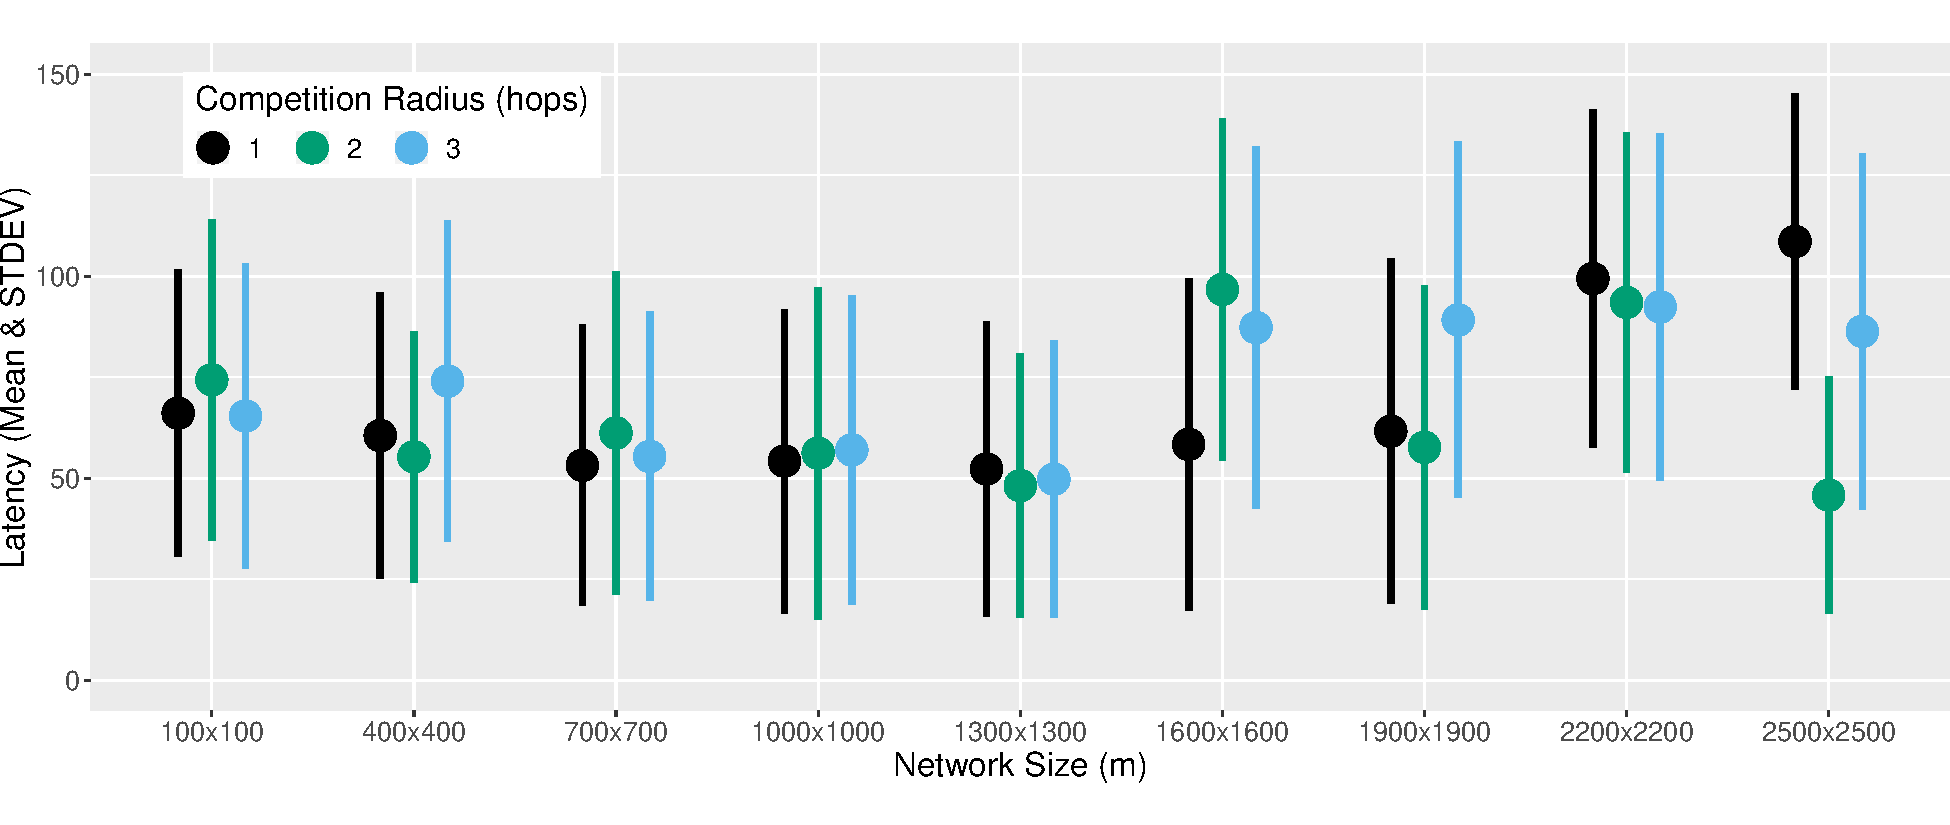
\includegraphics[width=\textwidth, keepaspectratio]{figure/Results/ParameterEvaluation/Latency/ResyncTreshold1_Latency.pdf}
    \caption{Re-synchronisation threshold 1.}
    \label{subfig:resync-treshold-1-latency}
\end{subfigure}
\begin{subfigure}{0.80\textwidth}
    \centering
    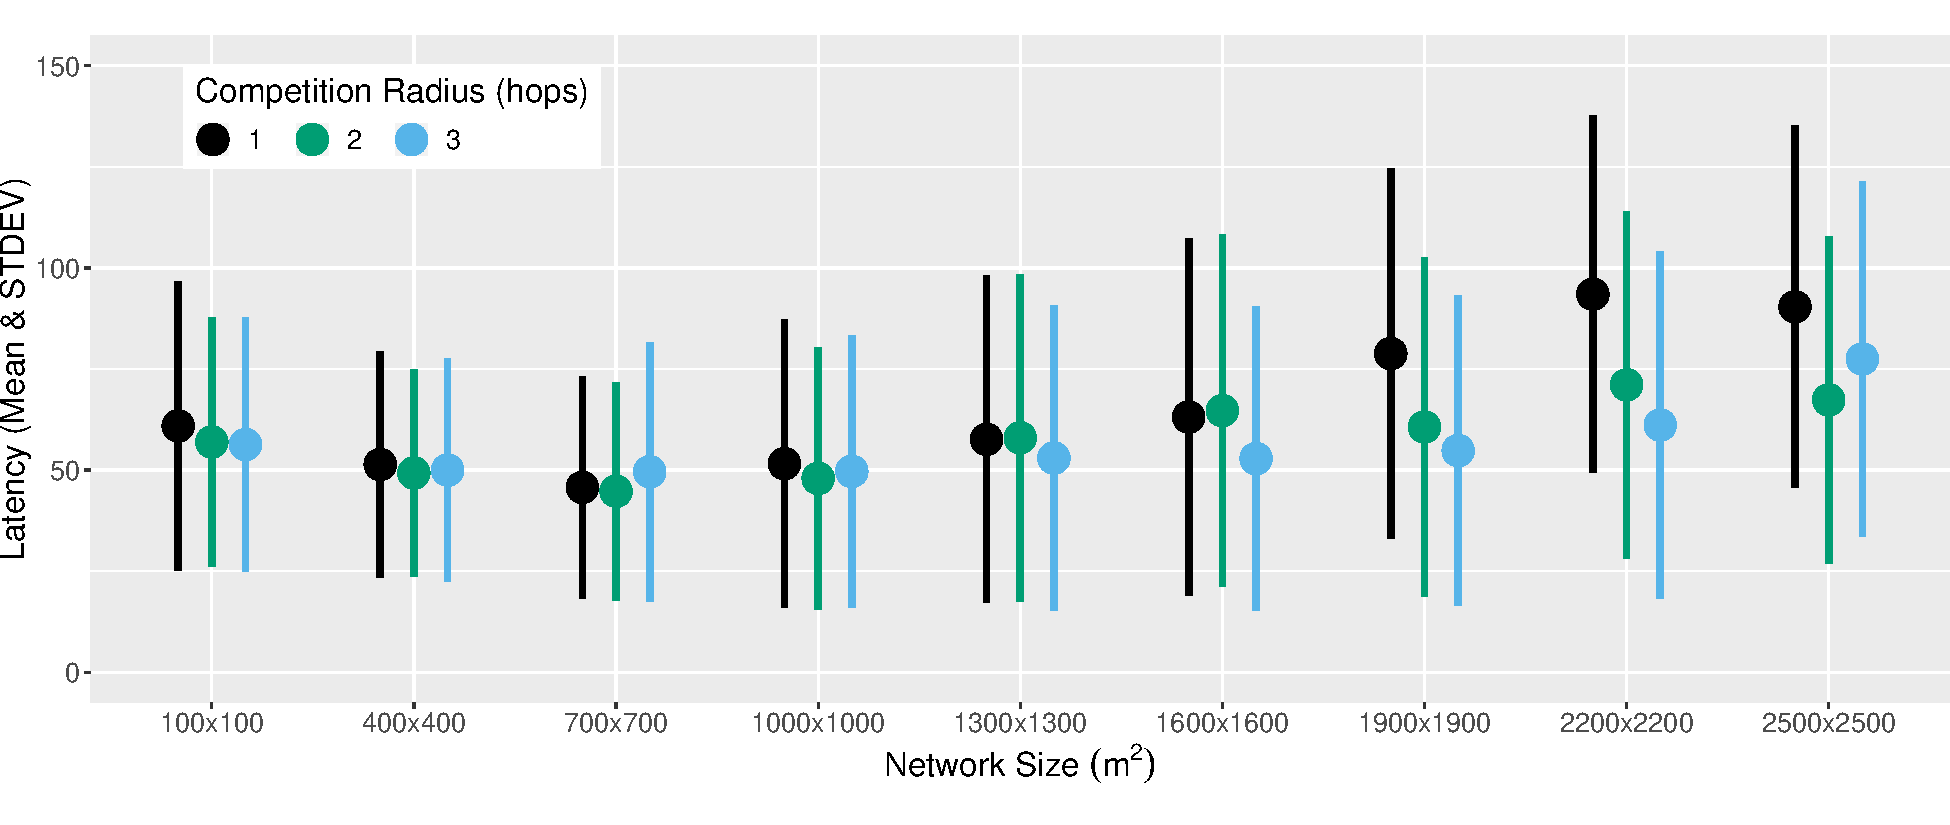
\includegraphics[width=\textwidth, keepaspectratio]{figure/Results/ParameterEvaluation/Latency/ResyncTreshold2_Latency.pdf}
    \caption{Re-synchronisation threshold 2.}
    \label{subfig:resync-treshold-2-latency}
\end{subfigure}
\begin{subfigure}{0.80\textwidth}
    \centering
    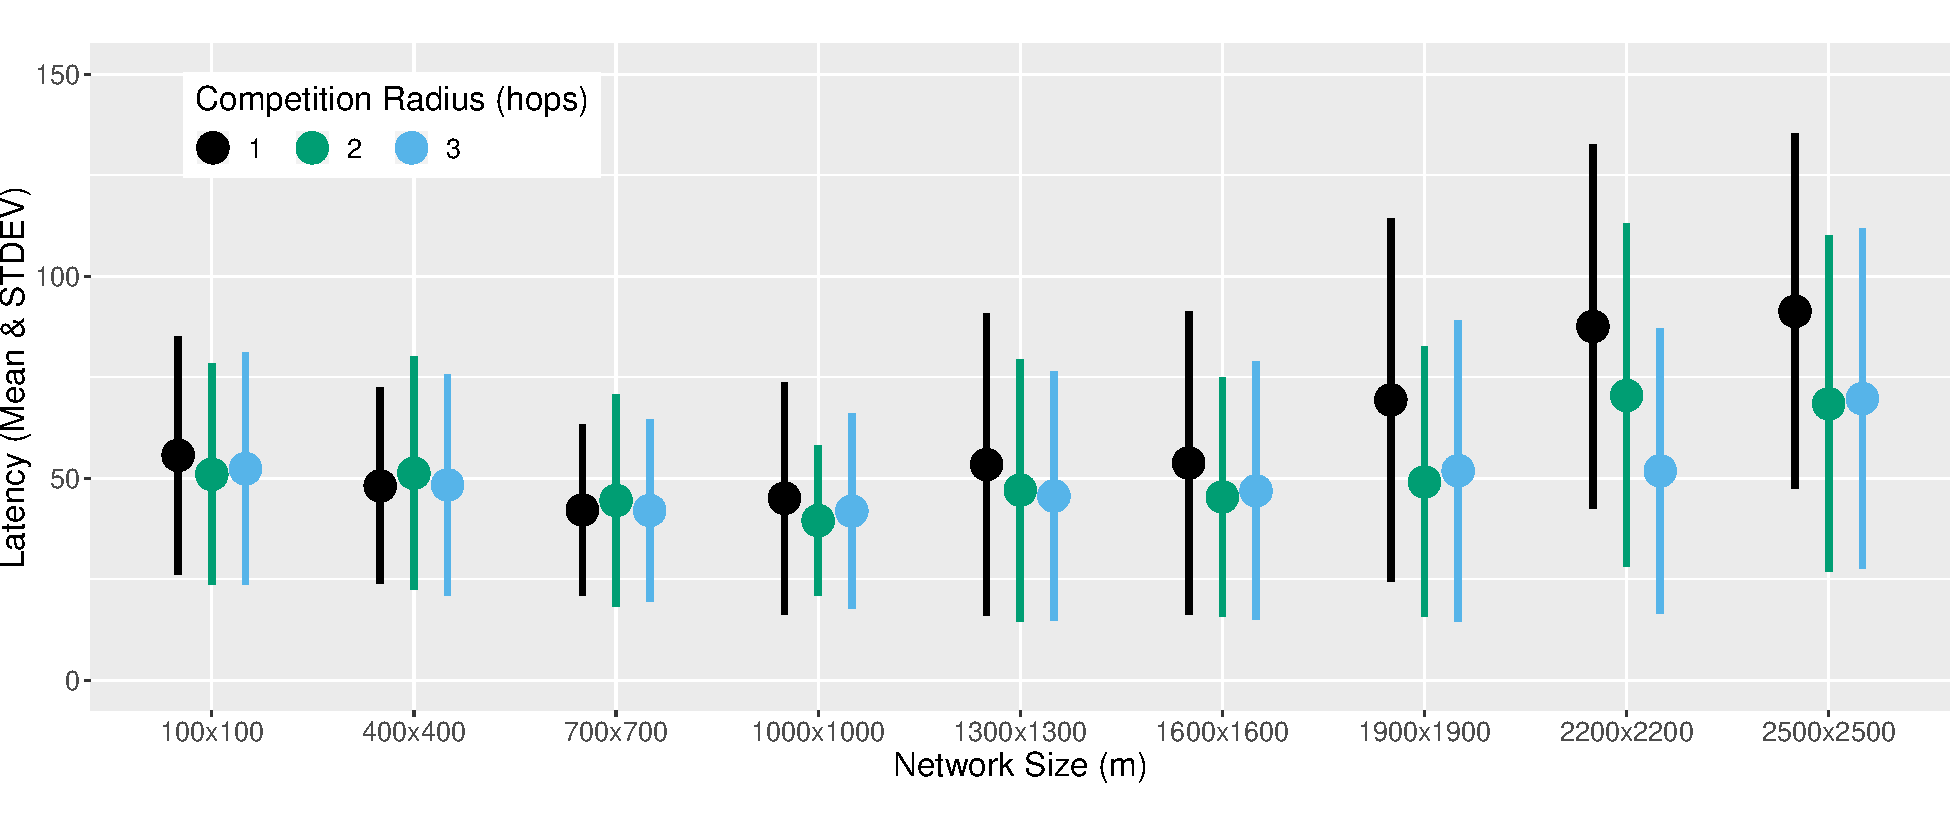
\includegraphics[width=\textwidth, keepaspectratio]{figure/Results/ParameterEvaluation/Latency/ResyncTreshold3_Latency.pdf}
    \caption{Re-synchronisation threshold 3.}
    \label{subfig:resync-treshold-3-latency}
\end{subfigure}

    \caption{Competition radii tests for different values of resynchronisation threshold.}
    \label{fig:resync-treshold-tests-latency}
\end{figure}

\section{Parameter Latency Plots}
\begin{figure}[H]
    
\centering
\begin{subfigure}{\textwidth}
    \centering
    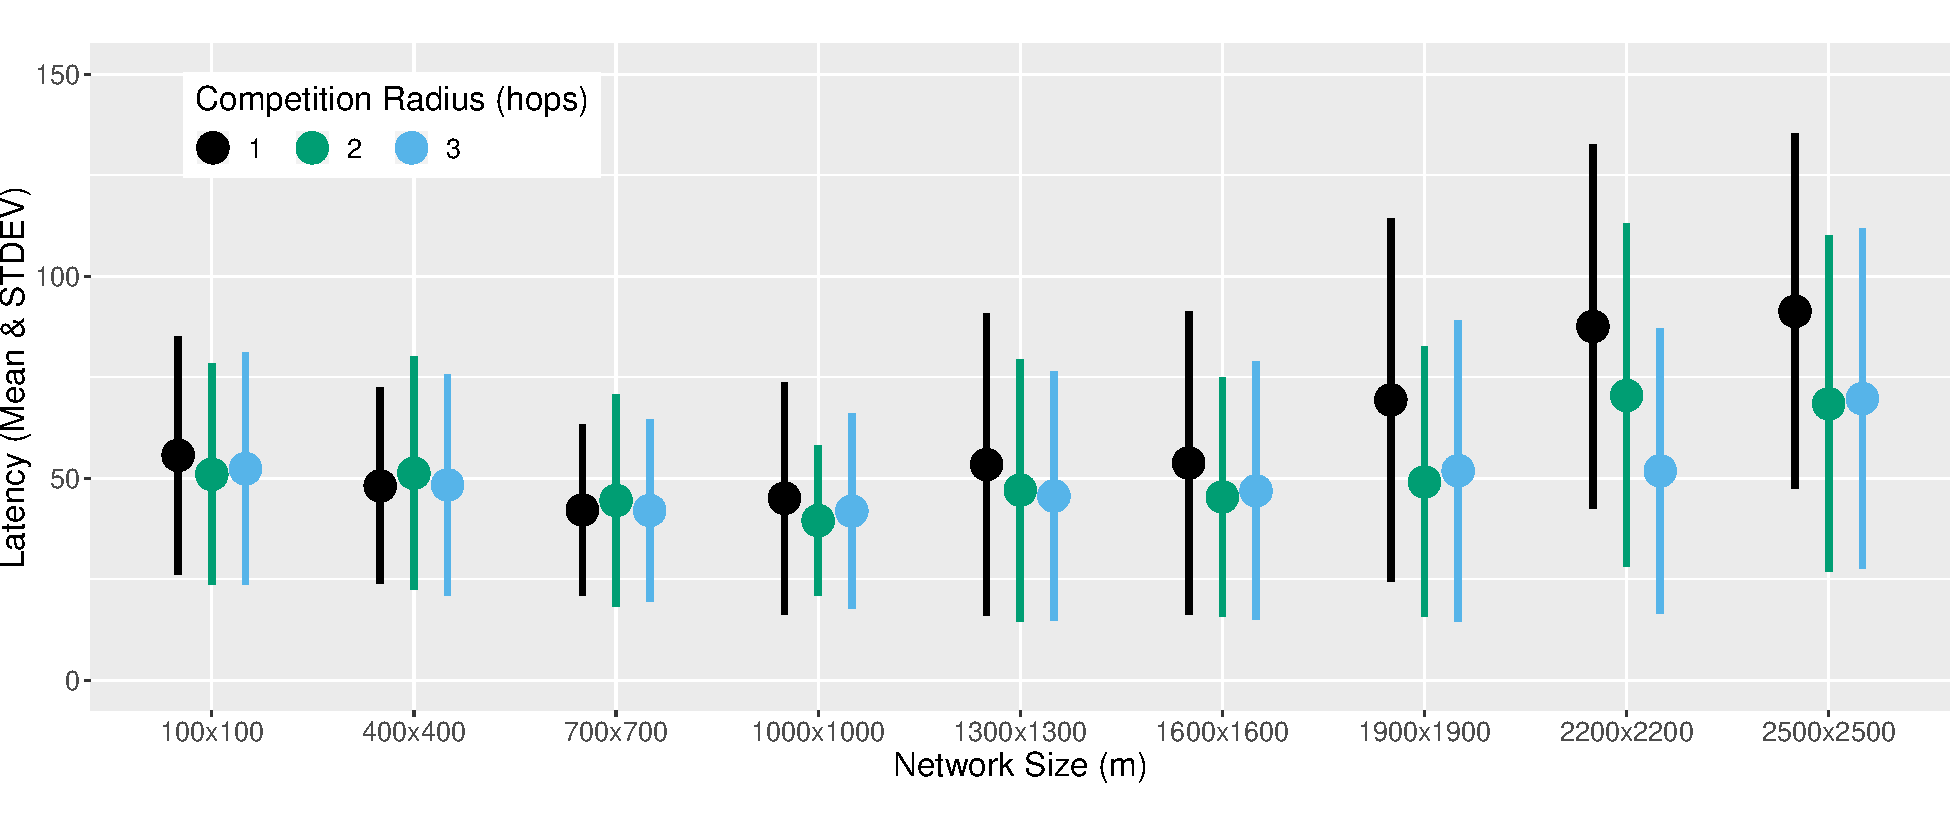
\includegraphics[width=\textwidth, keepaspectratio]{figure/Results/ParameterEvaluation/Latency/CompetitionRadius_Latency.pdf}
    \caption{Competition radius.}
    \label{subfig:competition-radius-latency}
\end{subfigure}
\begin{subfigure}{\textwidth}
    \centering
    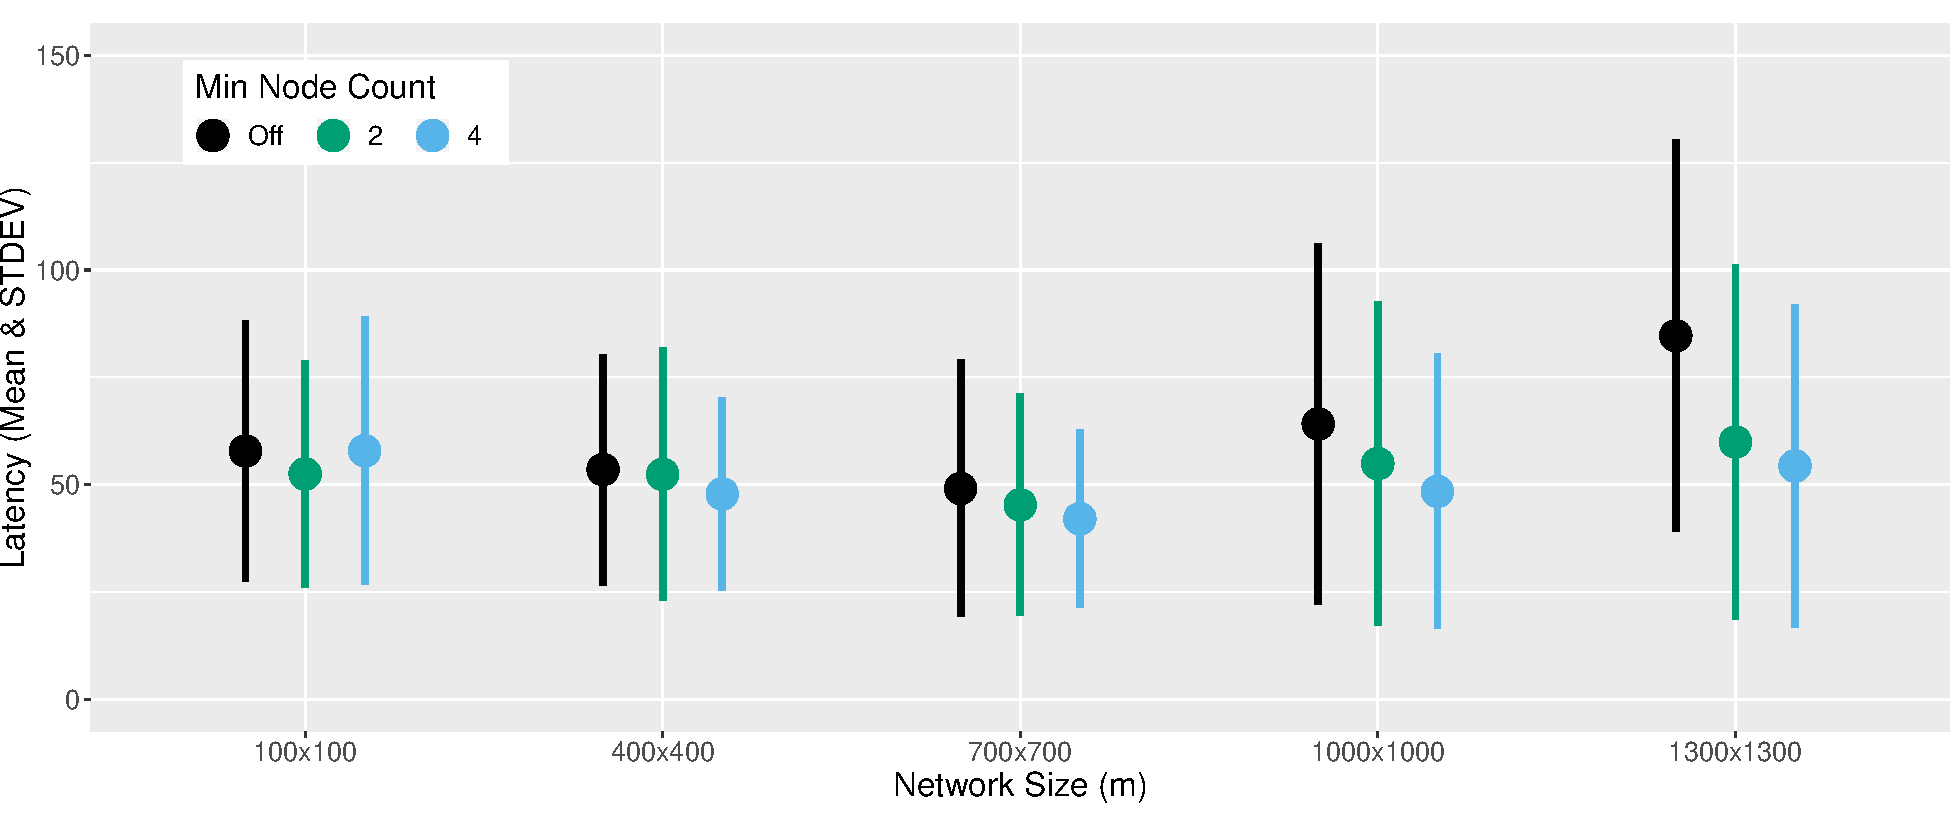
\includegraphics[width=\textwidth, keepaspectratio]{figure/Results/ParameterEvaluation/Latency/MinNodeCount_Latency.pdf}
    \caption{Minimum node count.}
    \label{subfig:min-node-count-latency}
\end{subfigure}
\begin{subfigure}{\textwidth}
    \centering
    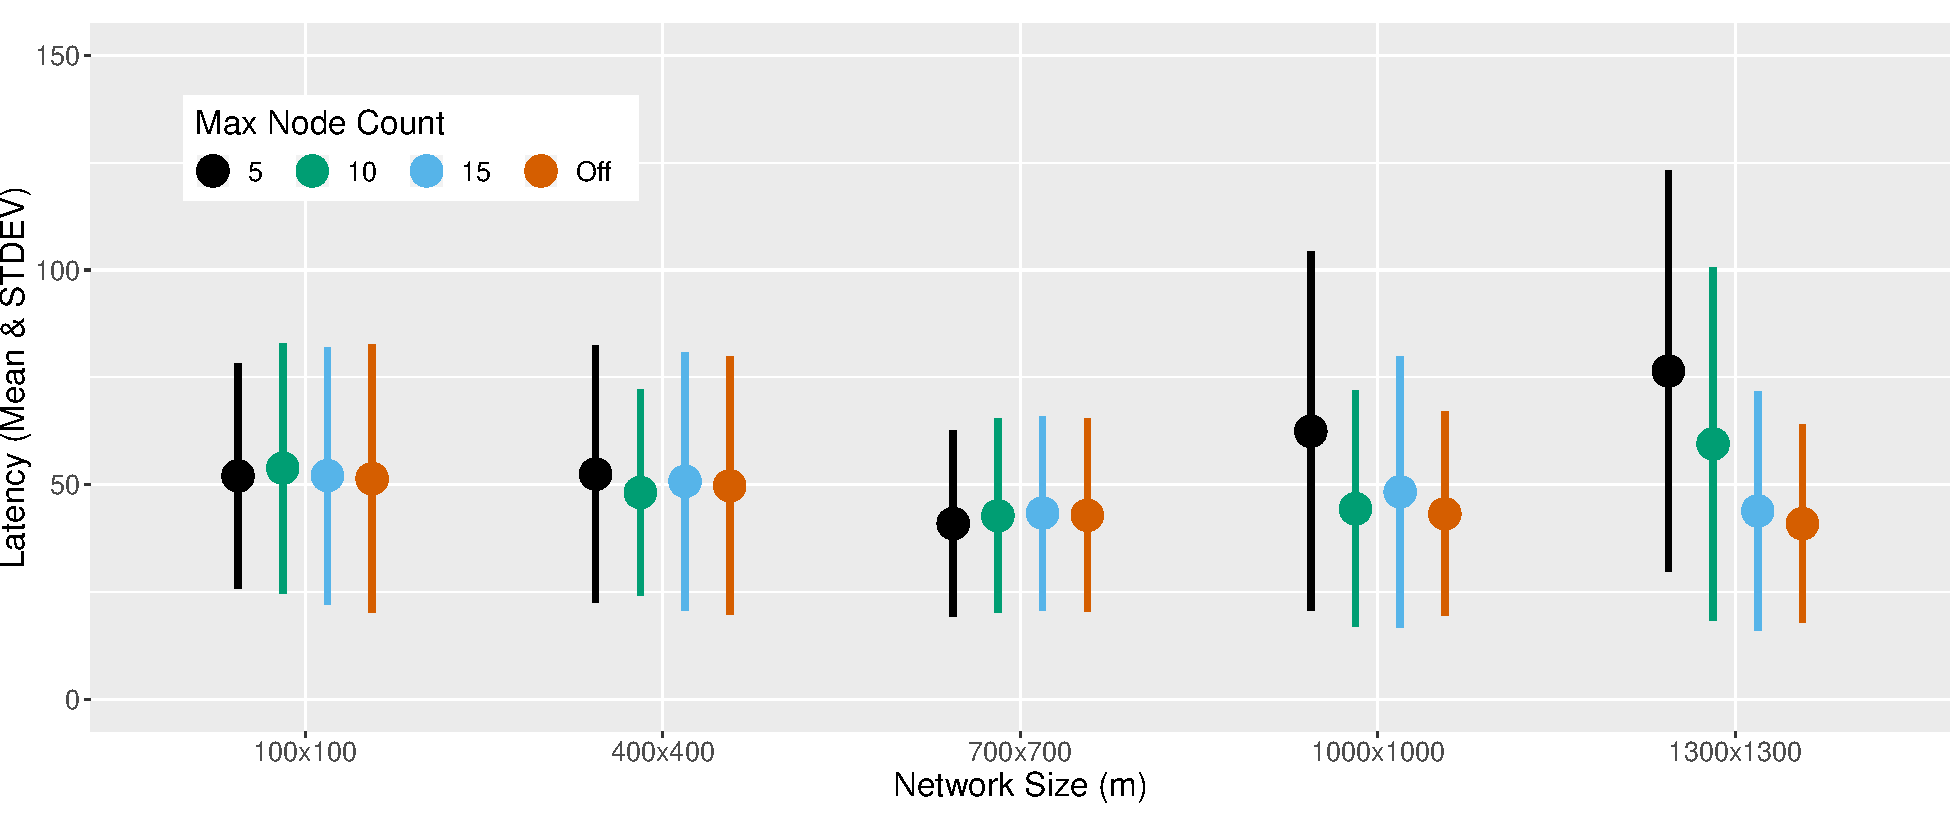
\includegraphics[width=\textwidth, keepaspectratio]{figure/Results/ParameterEvaluation/Latency/MaxNodeCount_Latency.pdf}
    \caption{Nodes per cluster ratio.}
    \label{subfig:max-node-count-latency}
\end{subfigure}

    \caption{The latency results for the parameter tests.}
    \label{fig:parameter-tests-latency}
\end{figure}

\chapter{Appendix 2}
\section{Parameter Values for the \atwo{} Comparison}
\label{app:parameter-values-for-the-atwo-comparison}
\begin{table}[H]
\centering
\caption{List of topologies with 50 nodes and the competition radius used for each topology.}
\label{tab:50-nodes-competition-radius-value}
\begin{tabular}{|r|l|l|l|l|}
\hline
\multicolumn{1}{|c|}{\textbf{Competition Radius}} & \multicolumn{4}{l|}{\textbf{Topologies}}                        \\ \hline
1                                                 & \multicolumn{4}{l|}{100x100, 400x400}                           \\ \hline
2                                                 & \multicolumn{4}{l|}{700x700, 1000x1000, 1300x1300}              \\ \hline
3                                                 & \multicolumn{4}{l|}{1600x1600, 1900x1900, 2200x2200, 2500x2500} \\ \hline
\end{tabular}
\end{table}

\begin{table}[H]
\centering
\caption{List of topologies with 200 nodes and the nodes per cluster ratio used for each topology.}
\label{tab:50-nodes-nodes-per-cluster-ratio-value}
\begin{tabular}{|r|l|}
\hline
\textbf{Nodes Per Cluster Ratio} & \textbf{Topologies}           \\ \hline
10                               & 100x100, 400x400              \\ \hline
30                               & 700x700, 1000x1000, 1300x1300 \\ \hline
\end{tabular}
\end{table}

%\chapter{Application Heat maps for Reliability Comparison}
%In these figures, x-axis represents rounds and therefore progression in time, each row on the y-axis represents one node. The colour of a cell indicates what application a node executed during that round.
%\begin{figure}[H]
    \centering
    \begin{subfigure}{\textwidth}
        \centering
        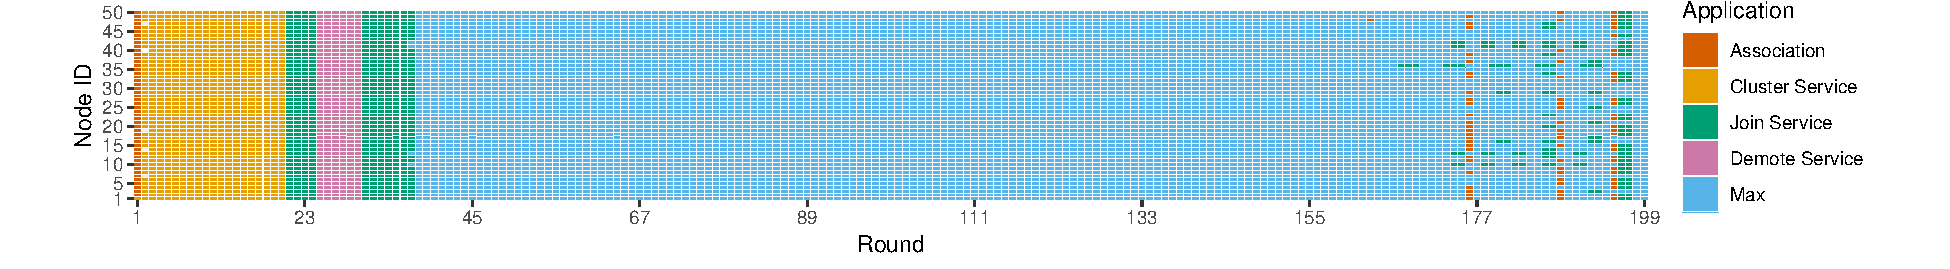
\includegraphics[width=\textwidth]{figure/Results/ReliabilityDiscussionApplicationHeatmaps/applicationmap50x50_1.pdf}
        \label{subfig:application-map-50-nodes-round-1-199}
    \end{subfigure}
    \hfill
    \begin{subfigure}{\textwidth}
        \centering
        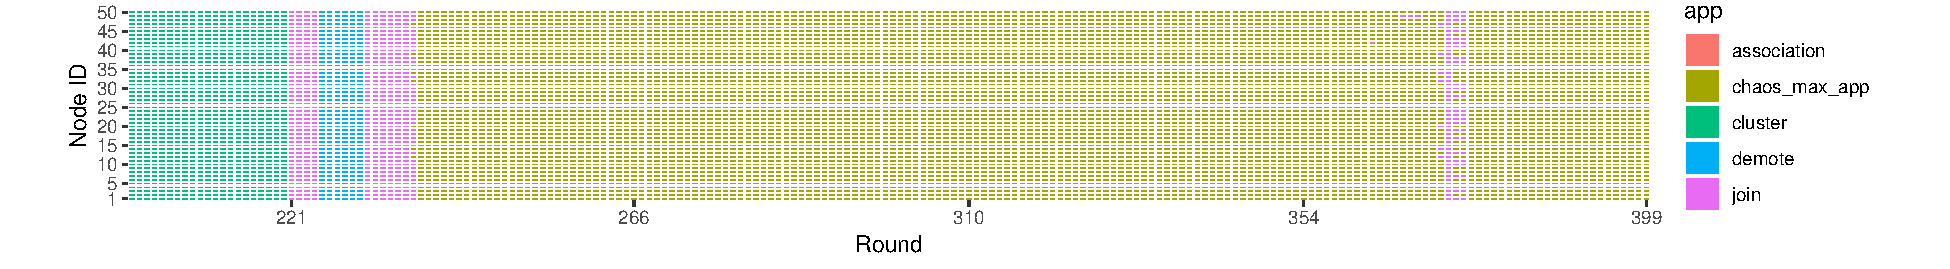
\includegraphics[width=\textwidth]{figure/Results/ReliabilityDiscussionApplicationHeatmaps/applicationmap50x50_2.pdf}
        \label{subfig:application-map-50-nodes-round-200-399}
    \end{subfigure}
    \begin{subfigure}{\textwidth}
        \centering
        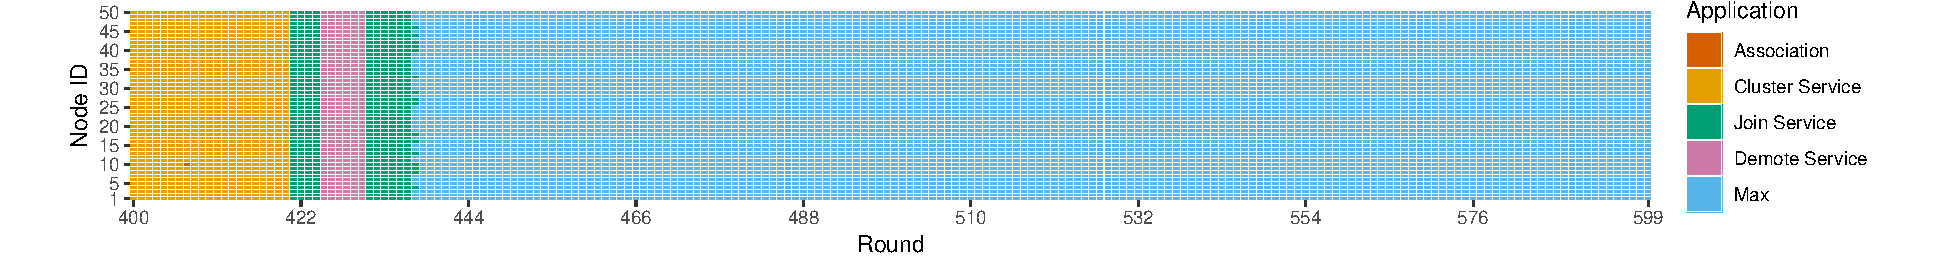
\includegraphics[width=\textwidth]{figure/Results/ReliabilityDiscussionApplicationHeatmaps/applicationmap50x50_3.pdf}
        \label{subfig:application-map-50-nodes-round-400-599}
    \end{subfigure}
    \caption{Application heat map of a test with 50 nodes over a 100x100 network area executing 600 rounds. Join is rarely executed outside its specified schedule.}
    \label{fig:application-map-50-nodes}
\end{figure}
%\begin{figure}[H]
\label{fig:application-map-200-nodes}
    \centering
    \begin{subfigure}{0.9\textwidth}
        \centering
        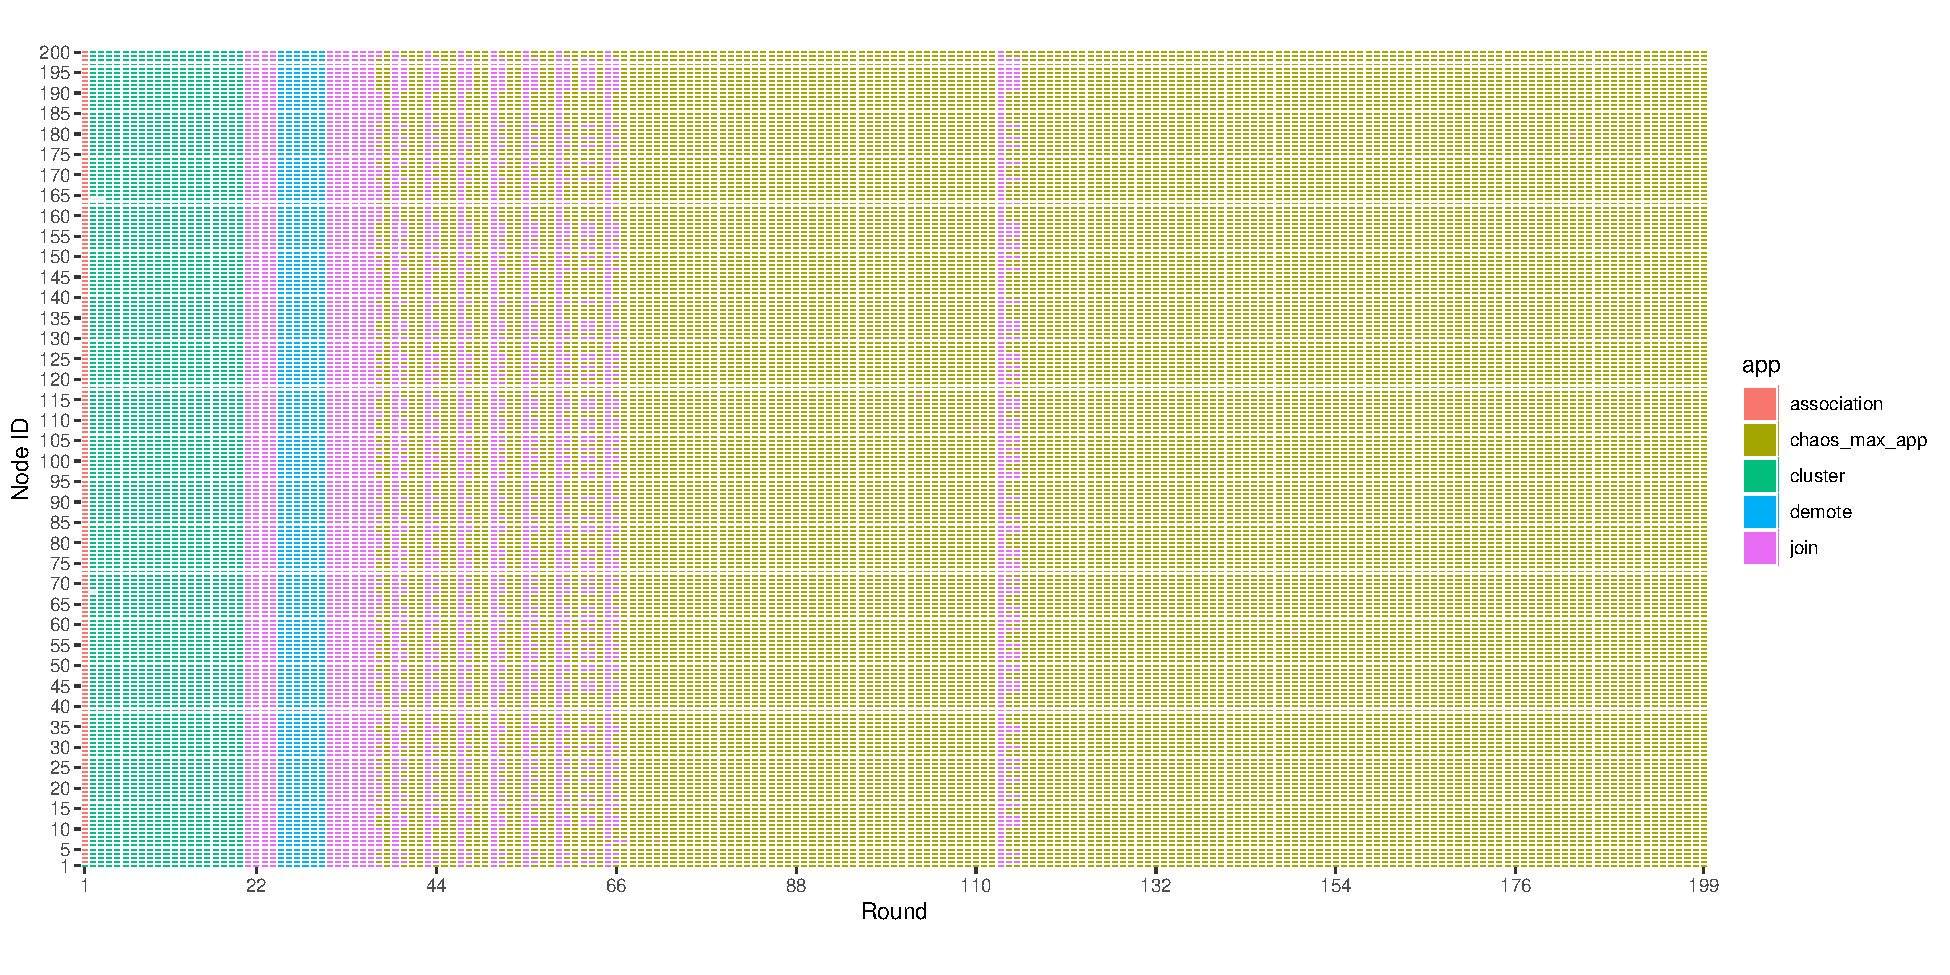
\includegraphics[width=\textwidth]{figure/Results/ReliabilityDiscussionApplicationHeatmaps/applicationmap200x200_1.pdf}
        \label{subfig:application-map-200-nodes-round-1-199}
    \end{subfigure}
    \hfill
    \begin{subfigure}{0.9\textwidth}
        \centering
        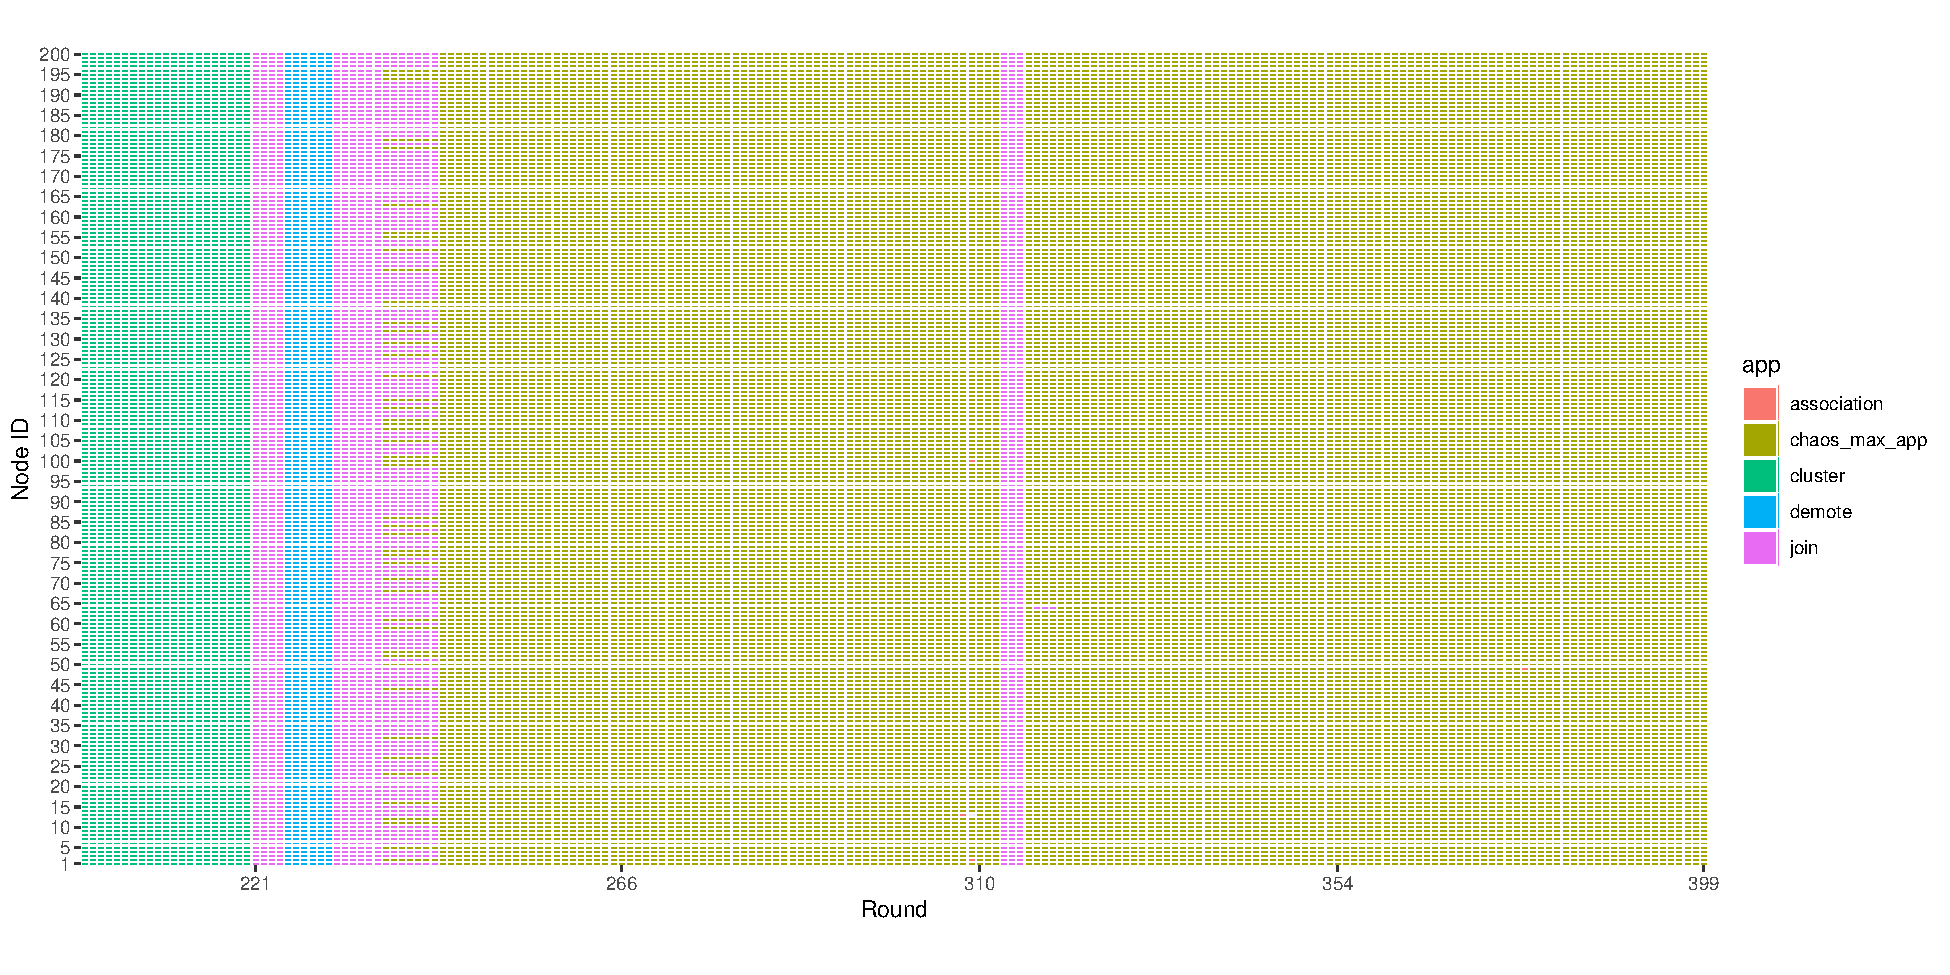
\includegraphics[width=\textwidth]{figure/Results/ReliabilityDiscussionApplicationHeatmaps/applicationmap200x200_2.pdf}
        \label{subfig:application-map-200-nodes-round-200-399}
    \end{subfigure}
    \begin{subfigure}{0.9\textwidth}
        \centering
        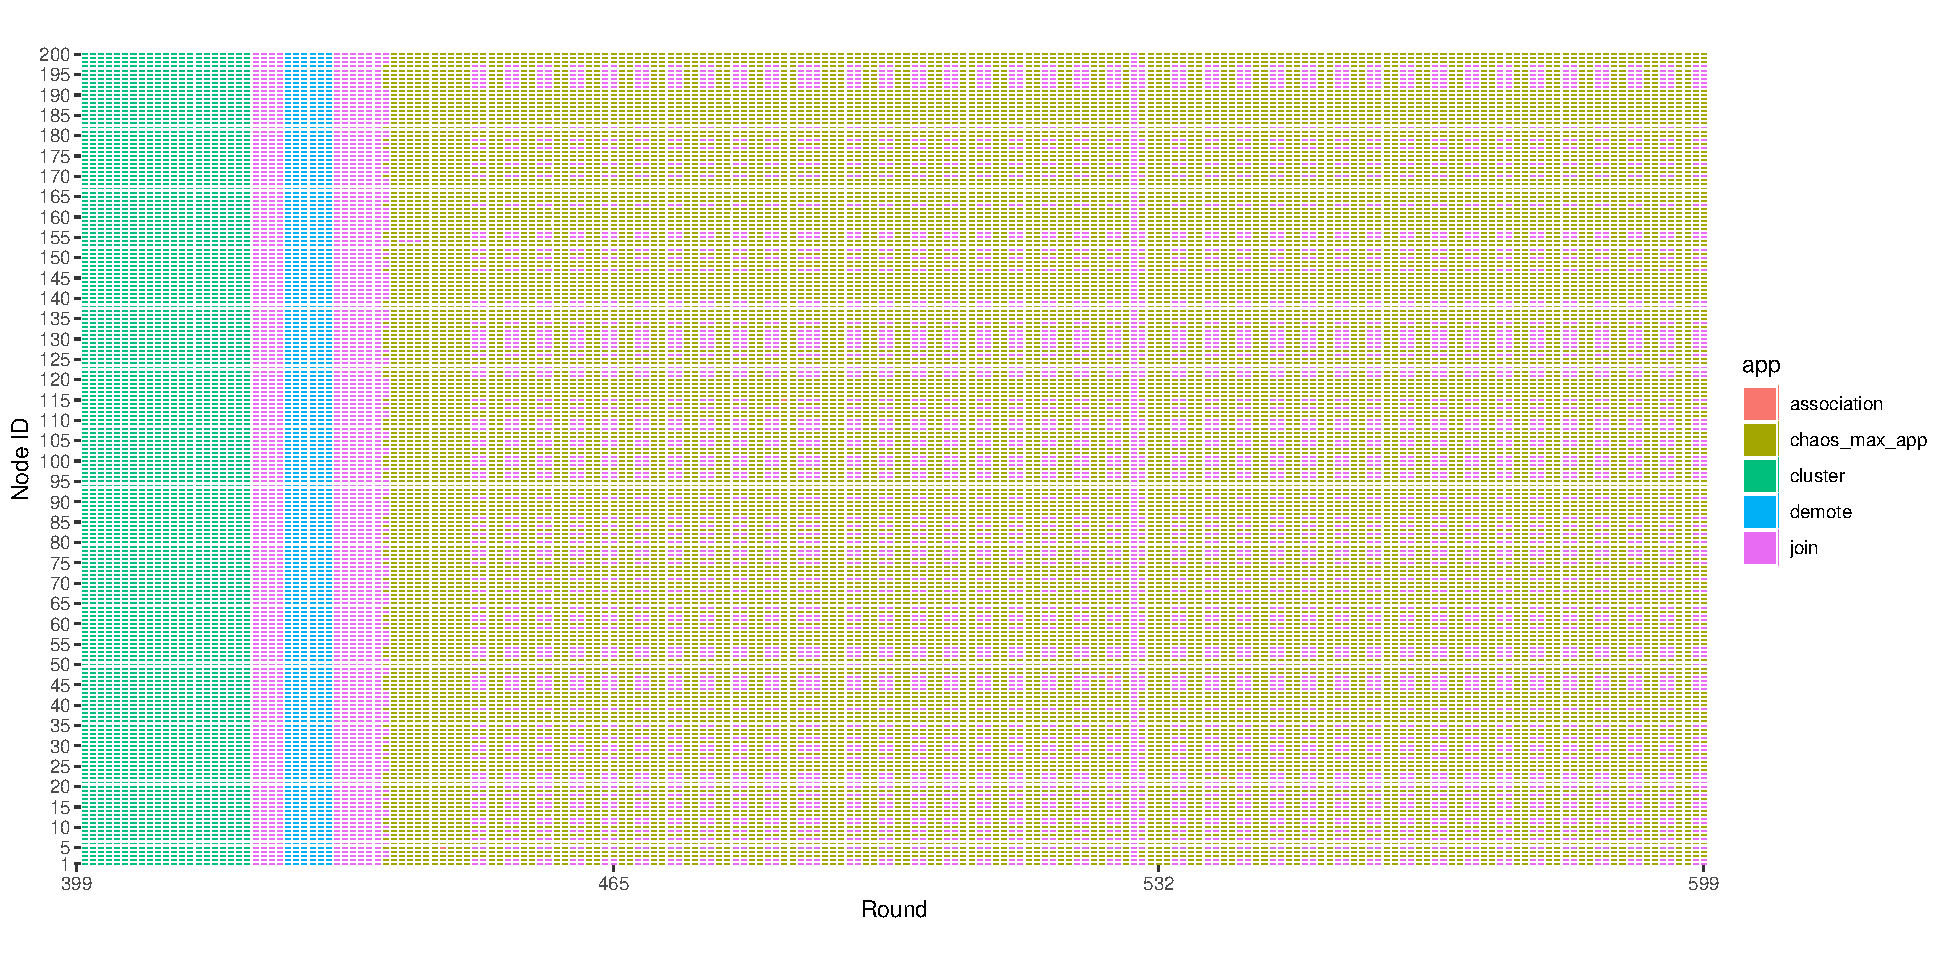
\includegraphics[width=\textwidth]{figure/Results/ReliabilityDiscussionApplicationHeatmaps/applicationmap200x200__3.pdf}
        \label{subfig:application-map-200-nodes-round-400-599}
    \end{subfigure}
    \caption{Application heat map of a test with 200 nodes over a 100x100 network area executing 600 rounds. Some clusters often execute join, especially after the last clustering occurring in rounds 400 to 437}
\end{figure}